\documentclass[tikz,border=2pt]{standalone}
\usepackage{amsmath,amssymb}
\usepackage{pgfplots}
\pgfplotsset{compat=1.18}

\begin{document}
% MGF of Exp(1), M(t) = 1/(1-t), near t = 0: the tangent has slope M'(0) = E[X] = 1 and the
% second-order approximation 1 + t + t^2 uses M''(0) = E[X^2] = 2.
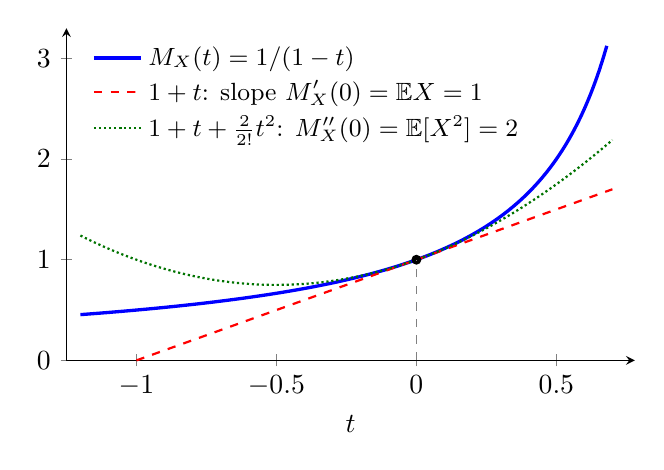
\begin{tikzpicture}
	\begin{axis}[
		axis lines=left, xmin=-1.25, xmax=0.78, ymin=0, ymax=3.3,
		xtick={-1,-0.5,0,0.5}, ytick={0,1,2,3},
		xlabel={$t$},
		samples=140, smooth, width=8.8cm, height=5.8cm, clip=false,
		legend style={draw=none, fill=none, font=\small, at={(0.03,0.98)}, anchor=north west}, legend cell align=left
		]
		\addplot[blue, very thick, domain=-1.2:0.68] {1/(1-x)};
		\addlegendentry{$M_X(t)=1/(1-t)$}
		\addplot[red, thick, dashed, domain=-1.0:0.7] {1+x};
		\addlegendentry{$1+t$: slope $M_X'(0)=\mathbb{E}X=1$}
		\addplot[green!45!black, thick, densely dotted, domain=-1.2:0.7] {1+x+x^2};
		\addlegendentry{$1+t+\tfrac{2}{2!}t^2$: $M_X''(0)=\mathbb{E}[X^2]=2$}
		\fill[black] (axis cs:0,1) circle (1.8pt);
		\draw[gray, dashed] (axis cs:0,0) -- (axis cs:0,1);
	\end{axis}
	
\end{tikzpicture}
\end{document}
